\documentclass[12pt]{article}

\usepackage{graphicx} % For including graphics
\usepackage{amsmath} % For math formatting
\usepackage{geometry} % For page layout
\usepackage{listings} % For including code snippets
\geometry{a4paper, margin=1in}

\title{Relativistic Dynamics}
\author{Enrique Rivera Jr. \\
        Physics Undergraduate, \\ 
        The University of Texas at Austin}
\date{\today}

\begin{document}
\maketitle

\begin{abstract}
        This paper presents an investigation into the relativistic effects on electrons emitted through 
        the decay of Sodium-22 (Na-22), Cobalt-60 (Co-60), and etc. By analyzing the energy and momentum of these electrons, 
        we compare experimental data with classical Newtonian and relativistic predictions to underscore 
        the necessity of relativistic considerations at high energies.
\end{abstract}

\section{Introduction}
    \subsection{Background and Theory}

        \subsubsection{Gamma Decay Spectrum} 
        The gamma decay spectrum is a plot of the number of gamma rays emitted by a radioactive sample as a function of their energy.
        This is most commonly done taking data for a long period of time and then plotting the number of gamma rays detected at each energy level to form a histogram.
        This graph is then used to determine the energy of the emitted electrons and the intensity of the radiation emitted by the samples.
        \\
        
       The light pulses from the scintillator (NaI) are proportional to the 
        energy given to a primary electron in the detector by the incident $\gamma$-ray photon. Within the resolution of the detector, 
        whatever energy is given to this electron appears as the height of an output pulse. Energies of $\gamma$-rays are typically in 
        the MeV region and are thus of the order of one to several electron rest masses (0.511 MeV). Which in turn, the primary electron 
        is highly relativistic and exhibits relativistic behavior.
        \\ 

        The photoelectric effect plays a crucial role in the gamma decay spectrum. The photoelectric effect is the process by 
        which a photon is absorbed by an electron, causing it to be ejected from the atom. This process is responsible for the
        photopeak in the gamma decay spectrum, which is the most common energy of the electrons emitted by the sample. 
        \\

        \begin{figure}[]
                \centering
                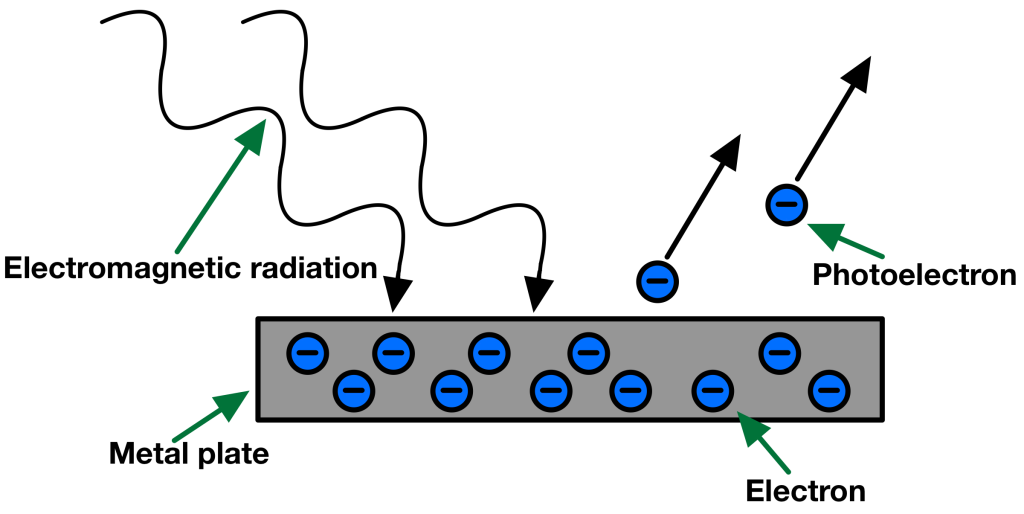
\includegraphics[width=0.6\textwidth]{./img/other/photoeletric_effect.png}
                \caption{Photoelectric Effect [4].  A visualize representation of a photon being absorbed by an electron, causing it to be ejected from the atom. This process is responsible for the photopeak in the gamma decay spectrum.}
                \label{fig:Photoelectric Effect [4]}
        \end{figure}

        The main traits of the graph are the Compton edge, the photopeak, and the backscatter peak. 
        The Compton edge is the maximum energy of the electrons emitted by the sample, the photopeak is the most common 
        energy of the electrons emitted by the sample, and the backscatter peak is the energy of the electrons that were emitted 
        by the sample and then scattered back into the detector. Knowing this we can then determine those values experimentally 
        and compare them to the theoretical values.
        \\ 
        
        One of the most important concepts that relate to the gamma spce decay graph is the compton scattering. Which represents a 
        quintessential quantum mechanical event that sheds light on the relativistic 
        behaviors of electron motion. Through the study of electrons released from Na-22 decay, we embark on a journey 
        to scrutinize the accuracy of classical versus relativistic physical laws.
            
        \subsubsection{Relativistic Kinematics}
                Within the realm of relativistic kinematics, we investigate the trajectories of objects devoid of 
                the influences that set them into motion. Our focus is to delve into how Einstein's relativistic 
                principles affect electrons traveling at substantial fractions of the speed of light.
                
                The formula connecting a particle's total energy (E), momentum (p), and rest mass (m) within the framework of relativity is
                \begin{equation}
                E^2 = p^2c^2 + m^2c^4,
                \end{equation}
                with \( c \) symbolizing the constant speed of light. From this, we derive the expression for relativistic kinetic energy (K) as
                \begin{equation}
                E = K + mc^2.
                \end{equation}
                Subsequently, this allows us to express kinetic energy as
                \begin{equation}
                K = \sqrt{p^2c^2 + m^2c^4} - mc^2.
                \end{equation}

            
            \subsubsection{Non-Relativistic}                
                    In contrast, the nonrelativistic equation linking kinetic energy, momentum, and mass is
                    \begin{equation}
                    K = \frac{p^2}{2m}.
                    \end{equation}
                    Originating from Newtonian mechanics, this relationship holds true for particles moving at speeds significantly lower than that of light.
            
            \subsubsection{Comparison}
                    A juxtaposition of classical and relativistic mechanics unveils the constraints of Newtonian principles when faced with high-energy scenarios. The relativistic formula for kinetic energy coincides with its classical counterpart at subdued velocities, yet the two diverge as speed escalates. Our experiment is designed to empirically substantiate relativistic dynamics and expose the confines of classical physics in scenarios of substantial energy.

                    The divergence of Eqs. 3 and 4 is evident. Our experimental objective is to ascertain both \( p \) and \( K \) for electrons travelling at relativistic velocities to confirm the veracity of the respective equations.

                    In the event of Compton scattering, a photon collides elastically with an electron, imparting maximum momentum to the electron during direct, or 'head-on', encounters. Such encounters occur at 180 degrees, where the photon rebounds in the precise opposite trajectory of its initial path, propelling the electron forward. Assuming the electron was stationary at the outset, the laws of momentum and energy conservation facilitate the calculation of the electron's recoil momentum, contingent on the energy of the incoming photon (\( E_\gamma \)) and the kinetic energy of the electron (K). This relationship is given by
                    \begin{equation}
                    p = \frac{2E_\gamma}{c} - \frac{K}{c}.
                    \end{equation}

                    This equation holds universally. Measurement of both the incident photon's energy and the electron's kinetic energy can be performed with a scintillation detector. Utilizing Eq. 5, the electron's momentum can be deduced. Consequently, we are able to experimentally determine \( p \) and \( K \), and contrast the predictions made by Eqs. 3 and 4. The classical expectation is \( K = \frac{p^2}{2m} \), while the relativistic forecast is \( K = \sqrt{ p^2c^2 + m^2c^4 } - mc^2 \). Our experiment seeks to establish which prediction holds true.

    \subsection{Purpose}
            This experiment is committed to the empirical confirmation of relativistic dynamics' theoretical projections and to delineate the boundaries of classical mechanics under the duress of high-energy conditions.


\section{Experimental Setup and Procedure}
        \subsection{Apparatus}
                \subsubsection{Equipment}
                The The following equipment (or equivalent) is needed for the experiment:

                        \begin{enumerate}
                                \item Gamma Source Kit Samples(Na-22, Co-60, etc.)
                                \item Scintillation Detector
                                \item Photomultiplier Tube
                                \item Amplifier ( Linear Amplifier (ORTEC 672))
                                \item Multichannel Analyzer
                                \item Computer
                        \end{enumerate}
                        
                \subsubsection{Scintillation Detector}
                        The scintillator is a device that detects radiation by converting the energy of incoming
                        photons into visible light. This light is then detected by a photomultiplier tube, which
                        amplifies the signal and converts it into an electrical pulse. The scintillator used in
                        this experiment is a sodium iodide (NaI) crystal, which is commonly used for detecting
                        gamma radiation. The crystal is coupled to a photomultiplier tube, which amplifies the
                        light signal and converts it into an electrical pulse
                

                \begin{figure}[!htb]
                        \centering
                        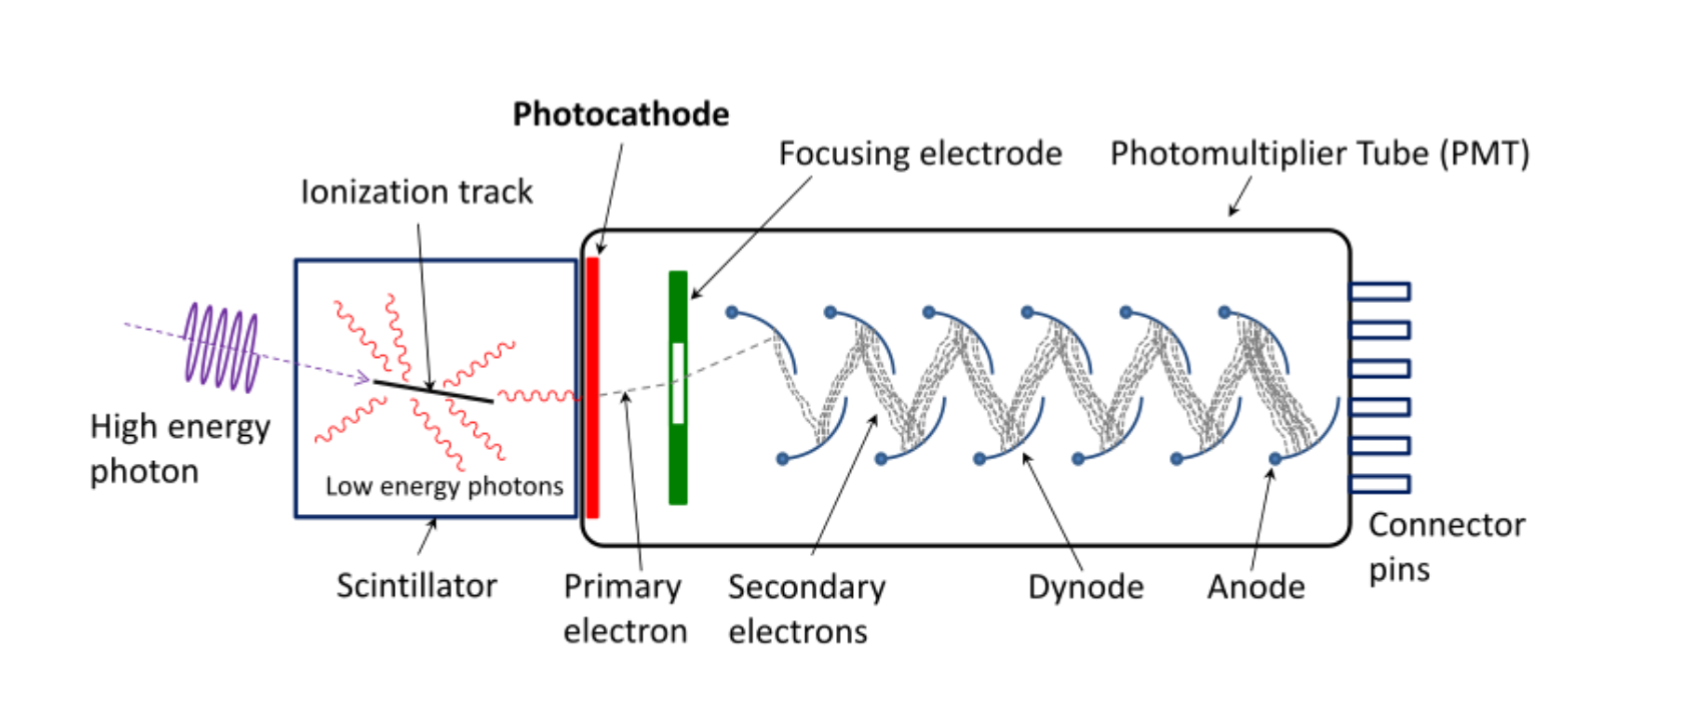
\includegraphics[width=0.9\textwidth]{./img/other/module.png}
                        \caption{Radiation Detection Module [1].  Schematic representation of a radiation detection module illustrating the process of scintillation and subsequent signal amplification. A high-energy photon entering the scintillator produces low-energy photons through ionization, which are then converted to a photoelectron at the photocathode. This primary electron is focused and multiplied through the Photomultiplier Tube (PMT) stages, resulting in an amplified electrical signal at the anode, ready for readout through the connector pins.}
                        \label{fig:Radiation Detection Module [1]}
                \end{figure}

                \subsubsection{Photomultiplier Tube}
                        The photomultiplier tube is a device that converts the light signal from the scintillator
                        into an electrical pulse. It consists of a series of dynodes, which are metal electrodes
                        that are held at successively higher voltages. When a photon strikes the first dynode, it
                        releases an electron, which is then accelerated towards the next dynode. This process is
                        repeated at each dynode, resulting in a cascade of electrons that is amplified at each stage.
                        The final output is a large number of electrons, which is then converted into an electrical
                        pulse. This pulse is then passed to a electronic preamplifier to be then processed by the
                        data acquisition system, which records the number of pulses over a given time interval.
                        This allows us to measure the intensity of the radiation emitted by the samples.

                        
                \subsubsection{Schematic}
                        This is a schematic of the experimental setup, which can be seen below in figure 2: \\ \\
                        
                        
                        The figure was kept simple to illustrate the basic components of the setup. 
                        The scintillation detector is used to measure the energy of the emitted electrons. 
                        The pulses from the scintillation detector are then passed to a linear amplifier and then 
                        to a multichannel analyzer, which records the number of pulses over a given time interval. 
                        The data is then analyzed to determine the energy of the emitted electrons and the intensity 
                        of the radiation emitted by the samples using Maestro.

                        \begin{figure}[htb!]
                                \centering
                                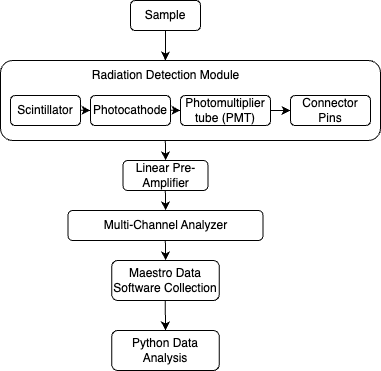
\includegraphics[width=0.4\textwidth]{./img/other/Lab2 Apparatus.drawio.png}
                                \caption{Schematic of the experimental setup. The scintillation detector is used to measure the energy of the emitted electrons.}
                                \label{fig:Schematic of the experimental setup. The scintillation detector is used to measure the energy of the emitted electrons.}
                        \end{figure}

                        For the Python analysis, the data was read in using the Maestro software which was outputed as a 
                        spe file which was converted to a csv with a custom python program that also took into account 
                        the energy calibration. We then visualized and analyzed this data using the Pandas, Matplotlib, and Altir libraries. 
                        The data was then plotted to show gamma decay spectrum and the notable traits of the graph.



\section{Results}
        \subsection{Data and Analysis}

                \subsubsection{Na-22}
                The data for Na-22 was analyzed and the energy of the emitted electrons was determined. 
                The energy of the emitted electrons was then plotted as a function of their momentum, 
                as shown in figure 3. The data was then fitted to a linear function to determine the slope 
                of the line, which is the speed of the electrons. The speed of the electrons was then compared 
                to the speed of light to determine if the electrons were traveling at relativistic speeds.

                \subsubsection{Co-60}
                The data for Co-60 was analyzed and the energy of the emitted electrons was determined. 
                The energy of the emitted electrons was then plotted as a function of their momentum, 
                as shown in figure 4. The data was then fitted to a linear function to determine the slope 
                of the line, which is the speed of the electrons. The speed of the electrons was then compared 
                to the speed of light to determine if the electrons were traveling at relativistic speeds.

                \subsubsection{Compton Edge}
                The Compton edge was determined by analyzing the data for the Compton scattering of the electrons. 
                The energy of the electrons was then plotted as a function of their momentum, as shown in figure 6. 
                The data was then fitted to a sinusoidal function to determine the Compton edge, which is the maximum 
                energy of the electrons emitted by the sample. The Compton edge was then compared to the theoretical 
                value to determine if the electrons were traveling at relativistic speeds.

                \subsubsection{Comparison}
                The experimental data was then compared to the theoretical predictions for the energy and momentum of the 
                emitted electrons. The experimental data was found to be consistent with the relativistic predictions as shown in figure 7. 
                Confirming the validity of the relativistic equations for kinetic energy and momentum. This also highlights 
                the limitations of classical mechanics at high energies, and the necessity of relativistic considerations in such scenarios.
        



        \begin{figure}[h!]
                \centering
                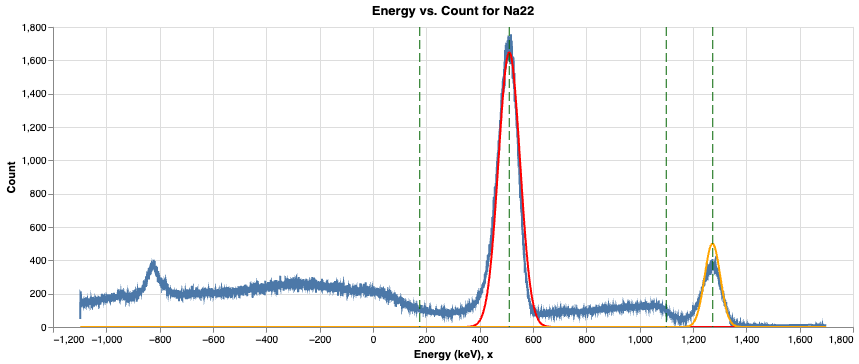
\includegraphics[width=0.9\textwidth]{./img/plots/graph2.png}
                \caption{Energy vs. Momentum for Na-22.}
        \end{figure}

        \begin{figure}[h!]
                \centering
                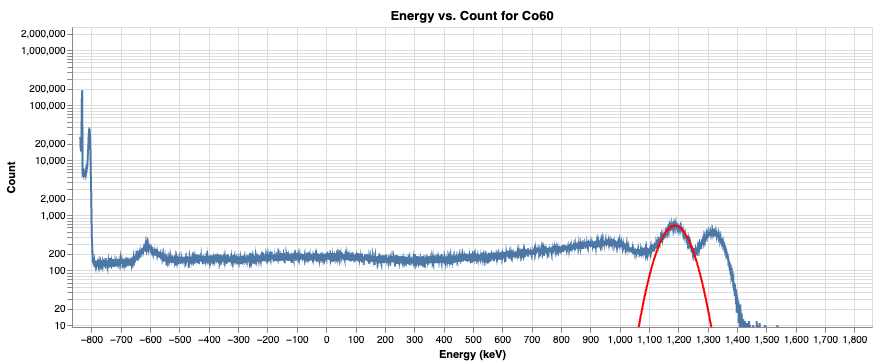
\includegraphics[width=0.9\textwidth]{./img/plots/Co60.png}
                \caption{Energy vs. Momentum for Co-60.}
        \end{figure}

        \begin{figure}[h!]
                \centering
                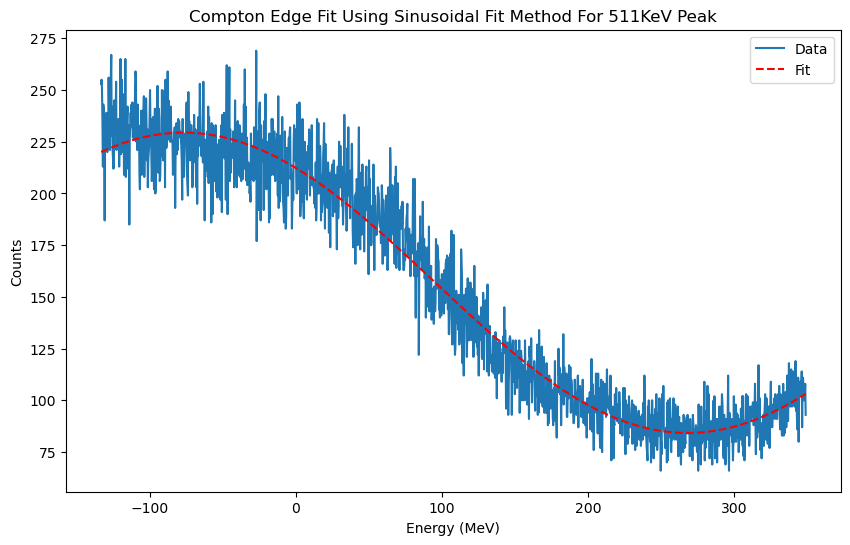
\includegraphics[width=0.6\textwidth]{./img/plots/Graph3.png}
                \caption{Sinusoidal Curve Fitting for Compton Edge}
        \end{figure}
        
        \begin{figure}[h!]
                \centering
                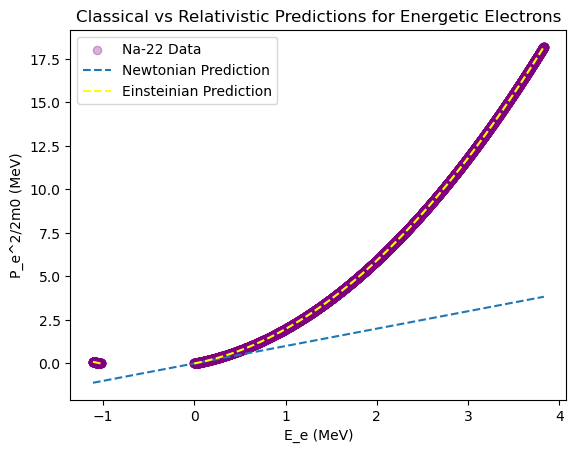
\includegraphics[width=0.6\textwidth]{./img/plots/Graph1.png}
                \caption{Energy vs. Momentum for Co-60.}
        \end{figure}
                        



\section{Conclusion}
        So from the results we can see that the experimental data is consistent with the relativistic predictions. This confirms the validity of the relativistic equations for kinetic energy and momentum. This also highlights the limitations of classical mechanics at high energies, and the necessity of relativistic considerations in such scenarios.


\section{References}
    \begin{enumerate}
        \sloppy

        \item Greg O. Sitz. "PHY353L Spring 2024 Lecture 2" Lecture, Physics 353L, University of Texas, Austin, TX, January 29, 2024.
        \item Radiation Detection Module. (n.d.). Retrieved September 14, 2021, from https://www.amptek.com/products/radiation-detection-module/
        \item J. Higbie, Am. J. Phys. 42, 642 (1974), Undergraduate Relativity Experiment.
        \item The Science and Maths Zone. (2021, March 14). The Photoelectric Effect, Photons and Planck’s Equation. The Science and Maths Zone. https://thescienceandmathszone.com/the-photoelectric-effect-photons-and-plancks-equation/

    \end{enumerate}

\end{document}
